\textit{长海今天人好多啊}
\subsection{题目描述}
Solve the 1D Schrödinger equation with the potential (i) \( V(x) = x^2 \); (ii) \( V(x) = x^4 - x^2 \) with the variational approach using a \textbf{Gaussian basis} (either fixed widths or fixed centers)
\[
    \phi_i(x)=(\frac{v_i}\pi)^{1/2} \mathrm{e}^{-v_i(x-s_i)^2}.
\]
Consider the three lowest energy eigenstates.

\subsection{程序描述}
本题要求用原版高斯基线性组合,通过变分原理找能级。高斯基并不相互正交,故需要计算重叠积分 $S_{ij}$:
\[
    S_{ij} = \left(\frac{v_i v_j}{v_i + v_j}\right)^{1/2} \exp{\left(-\frac{v_i v_j (s_i - s_j)^2}{v_i + v_j}\right)},
\]
接着计算动能积分 $T_{ij}$(此解答采用自然单位制 $\hbar = m = 1 $):
\[
    T_{ij} = \left(\frac{v_i^{3/2} v_j^{3/2}}{\sqrt{\pi} (v_i + v_j)^{5/2}}\right) \left[(v_i + v_j) - 2 v_i v_j (s_i - s_j)^2\right] \exp{\left(-\frac{v_i v_j (s_i - s_j)^2}{v_i + v_j}\right)}.
\]
而对于势能积分 $V_{ij}$,通过广义本征值问题 $\mathbf{H} \mathbf{c} = E \mathbf{S} \mathbf{c}$ 可以找到能级 $E$ 和对应的波函数 $\psi = \mathbf{c} \phi$。计算的难点在于,对于一般的势能 $V(x)$,高斯基下的积分
\[
    V_{ij} = \int \phi_i(x) V(x) \phi_j(x) \, dx
\]
没有解析解,需要数值积分来求解。幸运的是,本题所求的势能 $V(x)$ 是多项式形式,使用 Mathematica\textsuperscript{\textregistered} 可以方便地求解 $x^n$ 对应的势能积分。然而,高阶积分的解析表达式会变得非常复杂。GPT 提醒我,两个高斯基的乘积仍是一个新的高斯函数,因此可利用该特性来简化多项式势能的积分,即通过高斯分布的矩来处理。两个高斯函数的乘积为
\[
\phi_i(x) \phi_j(x) = \left(\frac{2 v_i v_j}{\pi^2}\right)^{1/4} \exp\left(-v_i (x - s_i)^2 - v_j (x - s_j)^2\right).
\]
将 $v_i (x - s_i)^2 + v_j (x - s_j)^2$ 展开为:
\[
(v_i + v_j) \left( x - \frac{v_i s_i + v_j s_j}{v_i + v_j} \right)^2 + \frac{v_i v_j (s_i - s_j)^2}{v_i + v_j}.
\]
因此,$\phi_i(x) \phi_j(x)$ 可以写成一个新的高斯函数的形式:
\[
\phi_i(x) \phi_j(x) = \left(\frac{2v_i v_j}{\pi (v_i + v_j)}\right)^{1/2} \exp\left(-\frac{v_i v_j (s_i - s_j)^2}{v_i + v_j}\right) \exp\left(- (v_i + v_j) \left(x - \mu\right)^2 \right),
\]
其中新的高斯分布的中心 $\mu$ 和方差 $\sigma^2$ 为:
\[
\mu = \frac{v_i s_i + v_j s_j}{v_i + v_j}, \quad \sigma^2 = \frac{1}{2(v_i + v_j)}.
\]
于是对于多项式形式的势能 $V(x) = x^n$,我们可以将势能积分转化为新高斯分布的矩问题。高斯分布 $G(x; \mu, \sigma^2)$ 的 $n$ 阶矩 $M_n = \mathbb{E}[x^n]$ 满足递推关系
\[
M_n(\mu, \sigma^2) = \mu M_{n-1}(\mu, \sigma^2) + (n-1) \sigma^2 M_{n-2}(\mu, \sigma^2),
\]
其中
\[
M_0 = 1, \quad M_1 = \mu.
\]
因此,前几个矩的具体值为
\[
M_2 = \mu^2 + \sigma^2,
\]
\[
M_3 = \mu^3 + 3 \mu \sigma^2,
\]
\[
M_4 = \mu^4 + 6 \mu^2 \sigma^2 + 3 \sigma^4.
\]
综上,势能积分可以表示为
\[
V_{ij} = S_{ij} \cdot M_n(\mu, \sigma^2),
\]
其中 $S_{ij}$ 是重叠积分,保证新高斯分布的归一化,$M_n$ 是高斯分布的 $n$ 阶矩。通过递推公式可以更方便地计算多项式势能下的高斯积分,\href{https://github.com/bud-primordium/Computational-Physics-Fall-2024/blob/main/Assignment_3/Problem_3/src/methods.jl#L106-L117}{源代码}中实际使用\texttt{Switch}语句处理了$n\in [1,4]$的情形。最后的本征值求解借助了\textit{Julia} \ \texttt{LinearAlgebra}库中的\texttt{eigen}函数,并采用梯形法计算最后波函数的归一化系数。

本题子目录结构如下
\begin{multicols}{2}
	\begin{verbatim}
        |-- Documenter.html
        |-- figs
        |-- problem_3.tex
        `-- src
            |-- documenter_output
            |-- integrals.nb
            |-- interaction.jl
            |-- main.jl
            |-- methods.jl
            `-- utils.jl
    \end{verbatim}
\end{multicols}
\noindent \textbf{助教老师}审阅源代码时,可借助\texttt{Documenter.html}便捷查看\texttt{Documenter}生成的\href{https://bud-primordium.github.io/Computational-Physics-Fall-2024/Assignment_3/Problem_3/src/documenter_output/build/index.html}{注释文档}。在\texttt{src}目录下,运行\ccmd{julia main.jl}即可运行程序(需安装\texttt{LinearAlgebra}与\texttt{Plots}包),\texttt{main.jl}是主程序入口点,其逻辑结构在伪代码 \ \ref{alg:interactive_entry} \ 中有详细说明;\texttt{methods.jl}负责算法实现,包括重叠积分,动能积分,势能积分与求解Schrödinger方程等,逻辑结构在伪代码 \ \ref{alg:integral_functions},\ref{alg:matrix_solver} \ 中有详细说明;\texttt{interaction.jl}负责交互功能,包括展示主菜单,根据不同选项处理用户输入输出等;\texttt{utils.jl}包含一些通用的工具函数,如梯形法,波函数归一化,异常处理等。目录下还准备了\texttt{integrals.nb},是用于验证高斯积分的 Mathematica\textsuperscript{\textregistered} 笔记本文件,最终源代码采用前述的多级矩计算方法,比直接录入Mathematica\textsuperscript{\textregistered}结果更加高效简洁且具备拓展性\footnote{猛然想起钟阳老师说DeepMD\textsuperscript{\textregistered}就是因为内置了许多积分查找的优化,速度提升不少。}。

程序主菜单提供了四个选项,分别对应使用:自定义参数求解题目要求的两种势阱、使用默认参数一次求解两种势阱,以及自定义四次以内的多项式势能进行求解。自定义参数包括高斯基数量、宽度$v$、中心$s$(在子模式下可选择变动其中之一,为另一个指定范围),输出能级数,自定义势阱系数等。用户还可以选择是否绘制波函数图像,但归一化处理较为耗时,故内置了多线程处理不同能级绘制,但依赖于用户授权,故建议至少使用\ccmd{julia -t 4 main.jl}运行,可显著提升绘图速度。输出结果与绘图详见\ref{sec:problem_3_example}节所示。

\textit{碎碎念:我多次尝试使用\texttt{PackageCompiler}打包编译本程序,奈何依赖屡屡出错,也没有合适的压缩方法,更不用谈交叉编译;尝试过使用\texttt{Pluto}交互式改造,发布至\textit{Binder},但新语法过多,中道崩殂。尽管我非常欣赏Julia超前的各项设计理念,风格优美在一众科学计算语言中当属清流,但生态实在还是不够配套,继续加油吧!}


\subsection{伪代码}
\begin{algorithm}[H]
    \caption{Interactive Entry Program for Solving the 1D Schrödinger Equation}
    \label{alg:interactive_entry}

    % Function and Data Format Settings
    \SetKwFunction{DisplayMenu}{DisplayMenu}
    \SetKwFunction{GetUserChoice}{GetUserChoice}
    \SetKwFunction{GetParameters}{GetParameters}
    \SetKwFunction{BuildMatrices}{BuildMatrices}
    \SetKwFunction{SolveSchrodinger}{SolveSchrodinger}
    \SetKwFunction{PrintEnergies}{PrintEnergies}
    \SetKwFunction{AskUserToPlot}{AskUserToPlot}
    \SetKwFunction{ComputeWavefunction}{ComputeWavefunction}
    \SetKwFunction{NormalizeWavefunction}{NormalizeWavefunction}
    \SetKwFunction{PlotWavefunctions}{PlotWavefunctions}
    \SetKwFunction{Range}{Range}
    \SetKwFunction{InitializeArray}{InitializeArray}
    \SetKwFunction{Print}{Print}

    \SetKwData{Choice}{choice}
    \SetKwData{Potential}{potential}
    \SetKwData{Params}{params}
    \SetKwData{PotentialName}{potential\_name}
    \SetKwData{NumLevels}{num\_levels}
    \SetKwData{XVals}{x\_vals}
    \SetKwData{Wavefunctions}{wavefunctions}
    \SetKwData{N}{N}
    \SetKwData{v}{v}
    \SetKwData{s}{s}
    \SetKwData{Energies}{energies}
    \SetKwData{States}{states}
    \SetKwData{PotentialList}{potential\_list}
    \SetKwData{ParamsList}{params\_list}
    \SetKwData{NameList}{name\_list}
    \SetKwData{HMatrix}{\textbf{H}}
    \SetKwData{SMatrix}{\textbf{S}}

    \KwIn{\ \Choice (str): User selection for potential type.\\
    \qquad \qquad \N (int): Number of basis functions.\\
    \qquad \qquad \v (Array[float]): Fixed or variable basis widths.\\
    \qquad \qquad \s (Array[float]): Basis center positions.\\
    \qquad \qquad \NumLevels (int) [default=3]: Number of energy levels to compute.}

    \KwOut{\Energies (Array), optional plots}

    \While{\textbf{True}}{
        \DisplayMenu()\tcp*[r]{Display menu options to the user}
        \Choice $\gets$ \GetUserChoice()\tcp*[r]{Get user's menu selection}

        \If{\Choice \textbf{equals} 'q' \textbf{or} \Choice \textbf{equals} 'Q'}{
            \Print("Program exited.")\tcp*[r]{Exit message}
            \textbf{break}\tcp*[r]{Terminate the loop}
        }

        (\N, \v, \s, \PotentialList, \ParamsList, \NameList, \NumLevels) $\gets$ \GetParameters(\Choice)\;
        \tcp{Option 1: Custom parameters for $V(x) = x^2$}
        \tcp{Option 2: Custom parameters for $V(x) = x^4 - x^2$}
        \tcp{Option 3: Use default parameters for both problems}
        \tcp{Option 4: Custom polynomial potential up to degree 4}

        \For{$i \gets 1$ \KwTo \texttt{Length}(\PotentialList)}{
            (\Potential, \Params, \PotentialName) $\gets$ (\PotentialList$[i]$, \ParamsList$[i]$, \NameList$[i]$)\;
            \tcp{Get potential function and its parameters}

            (\HMatrix, \SMatrix) $\gets$ \BuildMatrices(\N, \v, \s, \Potential, \Params)\tcp*[r]{Construct \HMatrix and \SMatrix matrices}

            (\Energies, \States) $\gets$ \SolveSchrodinger(\HMatrix, \SMatrix, \NumLevels)\tcp*[r]{Solve the eigenvalue problem}

            \PrintEnergies(\Energies, \PotentialName, \NumLevels)\tcp*[r]{Output energy levels}

            \If{\AskUserToPlot(\PotentialName)}{
                \XVals $\gets$ \Range($-5$, $5$, $200$)\;
                \Wavefunctions $\gets$ \InitializeArray(\NumLevels)\tcp*[r]{Prepare storage for wavefunctions}

                \For{$n \gets 1$ \KwTo \NumLevels}{
                    $\psi_n$ $\gets$ \ComputeWavefunction(\XVals, \States$[:, n]$, \v, \s, \N)\tcp*[r]{Compute wavefunction $\psi_n$}

                    \Wavefunctions$[n]$ $\gets$ \NormalizeWavefunction(\XVals, $\psi_n$)
                    \tcp*[r]{Using \textbf{trapezoidal method}}
                }
                \PlotWavefunctions(\XVals, \Wavefunctions, \NumLevels, \PotentialName, \Params)
            }
        }
    }
\end{algorithm}

\begin{algorithm}[H]
    \caption{Integral Functions for Gaussian Basis}
    \label{alg:integral_functions}

    % Function and Data Format Settings
    \SetKwProg{Fn}{Function}{:}{end}
    \SetKwFunction{OverlapIntegral}{OverlapIntegral}
    \SetKwFunction{KineticIntegral}{KineticIntegral}
    \SetKwFunction{PotentialIntegral}{PotentialIntegral}
    \SetKwFunction{ComputeMoment}{ComputeMoment}

    % Define Variables
    \SetKwData{Vp}{$v_p$}
    \SetKwData{Exponent}{$exponent$}
    \SetKwData{Prefactor}{$prefactor$}
    \SetKwData{Sij}{$S_{ij}$}
    \SetKwData{Tij}{$T_{ij}$}
    \SetKwData{Vij}{$V_{ij}$}
    \SetKwData{Mu}{$\mu$}
    \SetKwData{Sigma}{$\sigma^2$}
    \SetKwData{Mn}{$M_n$}

    % Mathematical Upright e
    \newcommand{\me}{\mathrm{e}}

    % Algorithms

    \Fn{\OverlapIntegral{$v_1$, $s_1$, $v_2$, $s_2$}}{
        \Vp $\gets v_1 + v_2$\tcp*[r]{Combined width parameter}
        \Exponent, \Prefactor $\gets - \dfrac{v_1 v_2 (s_1 - s_2)^2}{\Vp},\ \dfrac{\sqrt{v_1 v_2}}{\sqrt{\pi \Vp}}$\tcp*[r]{Exponent and prefactor}
        \Sij $\gets$ \Prefactor $\times$ $\me^{\Exponent}$\tcp*[r]{Compute overlap integral}
        \Return \Sij\;
    }

    \Fn{\KineticIntegral{$v_1$, $s_1$, $v_2$, $s_2$}}{
        \Vp $\gets v_1 + v_2$\tcp*[r]{Combined width parameter}
        \Exponent, \Prefactor $\gets - \dfrac{v_1 v_2 (s_1 - s_2)^2}{\Vp},\ \dfrac{v_1^{1.5} v_2^{1.5}}{\sqrt{\pi} \Vp^{2.5}}$\tcp*[r]{Exponent and prefactor}
        $numerator \gets \Vp - 2 v_1 v_2 (s_1 - s_2)^2$\tcp*[r]{Numerator in kinetic integral}
        \Tij $\gets$ \Prefactor $\times$ $numerator$ $\times$ $\me^{\Exponent}$\tcp*[r]{Compute kinetic energy integral}
        \Return \Tij\;
    }

    \Fn{\PotentialIntegral{$v_1$, $s_1$, $v_2$, $s_2$, $n$}}{
        \Vp $\gets v_1 + v_2$\tcp*[r]{Combined width parameter}
        \Exponent $\gets - \dfrac{v_1 v_2 (s_1 - s_2)^2}{\Vp}$\;
        \Sij $\gets \dfrac{\sqrt{v_1 v_2}}{\sqrt{\pi \Vp}} \times \me^{\Exponent}$\tcp*[r]{Compute overlap integral}
        \Mu $\gets \dfrac{v_1 s_1 + v_2 s_2}{\Vp}$\tcp*[r]{Mean of combined Gaussian}
        \Sigma $\gets \dfrac{1}{2 \Vp}$\tcp*[r]{Variance of combined Gaussian}
        \Mn $\gets$ \ComputeMoment{$n$, \Mu, \Sigma}\tcp*[r]{Compute the $n$-th moment}
        \Vij $\gets$ \Sij $\times$ \Mn\tcp*[r]{Compute potential energy integral}
        \Return \Vij\;
    }

    \Fn{\ComputeMoment{$n$, \Mu, \Sigma}}{
        \eIf{$n = 0$}{
            \Return $1$\tcp*[r]{Compute $M_n$ using moments of the normal distribution}
        }{
            \Return $\sum_{k=0}^{n} \binom{n}{k} \mu^{n-k} \sigma^{k} \cdot (n-k-1)!!$\tcp*[r]{General formula for $M_n$}
        }
    }

\end{algorithm}

\begin{algorithm}[H]
    \caption{Matrix Construction and Schrödinger Equation Solver}
    \label{alg:matrix_solver}

    % Function and Data Format Settings
    \SetKwProg{Fn}{Function}{:}{end}
    \SetKwFunction{BuildMatrices}{BuildMatrices}
    \SetKwFunction{SolveSchrodinger}{SolveSchrodinger}
    \SetKwFunction{OverlapIntegral}{OverlapIntegral}
    \SetKwFunction{KineticIntegral}{KineticIntegral}
    \SetKwFunction{PotentialFunction}{PotentialFunction}
    \SetKwFunction{GeneralizedEigenSolve}{GeneralizedEigenSolve}

    % Define Variables
    \SetKwData{HMatrix}{$\mathbf{H}$}
    \SetKwData{SMatrix}{$\mathbf{S}$}
    \SetKwData{Energies}{$energies$}
    \SetKwData{States}{$states$}
    \SetKwData{NumLevels}{$num\_levels$}
    \SetKwData{Idx}{$idx$}

    % Algorithms

    \Fn{\BuildMatrices{$N$, $v$, $s$, PotentialFunction, PotentialParams}}{
        Initialize \HMatrix\ and \SMatrix\ as $N \times N$ zero matrices\;
        \For{$i \gets 1$ \KwTo $N$}{
            \For{$j \gets i$ \KwTo $N$}{
                $S_{ij} \gets$ \OverlapIntegral{$v[i]$, $s[i]$, $v[j]$, $s[j]$}\;
                $T_{ij} \gets$ \KineticIntegral{$v[i]$, $s[i]$, $v[j]$, $s[j]$}\;
                $V_{ij} \gets$ \PotentialFunction($v[i]$, $s[i]$, $v[j]$, $s[j]$, PotentialParams)\;
                \HMatrix$[i, j] \gets T_{ij} + V_{ij}$\;
                \SMatrix$[i, j] \gets S_{ij}$\;
                \If{$i \ne j$}{
                    \HMatrix$[j, i],$ \SMatrix$[j, i] \gets$ \HMatrix$[i, j],$ \SMatrix$[i, j]$\tcp*[r]{Copy symmetric elements}
                }
            }
        }
        \Return \HMatrix, \SMatrix\;
    }

    \Fn{\SolveSchrodinger{\HMatrix, \SMatrix, \NumLevels}}{
        $(E\_values, E\_vectors) \gets$ \GeneralizedEigenSolve{\HMatrix, \SMatrix}\tcp*[r]{Solve $\mathbf{H} \mathbf{c} = E \mathbf{S} \mathbf{c}$}
        \Idx $\gets$ Indices that sort $E\_values$ in ascending order\;
        \Energies $\gets E\_values[\Idx[1..\NumLevels]]$\tcp*[r]{Select lowest \NumLevels\ energies}
        \States $\gets E\_vectors[:, \Idx[1..\NumLevels]]$\tcp*[r]{Corresponding eigenvectors}
        \Return \Energies, \States\;
    }

\end{algorithm}


\subsection{结果示例}
\label{sec:problem_3_example}
\begin{figure}[H]
	\centering
	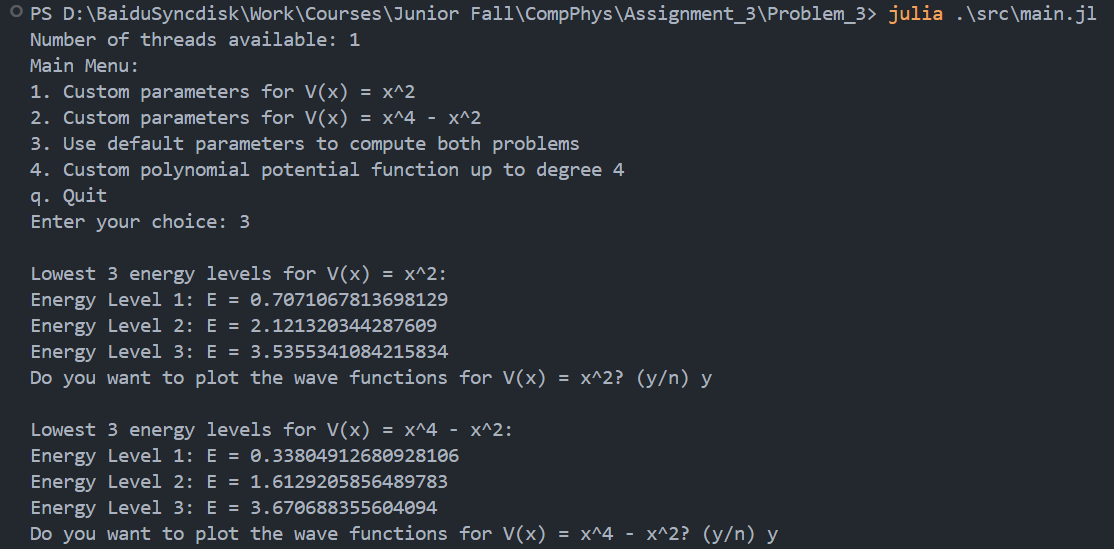
\includegraphics[width=0.8\textwidth]{Problem_3/figs/choice_3.png}
    \hspace{5pt}
    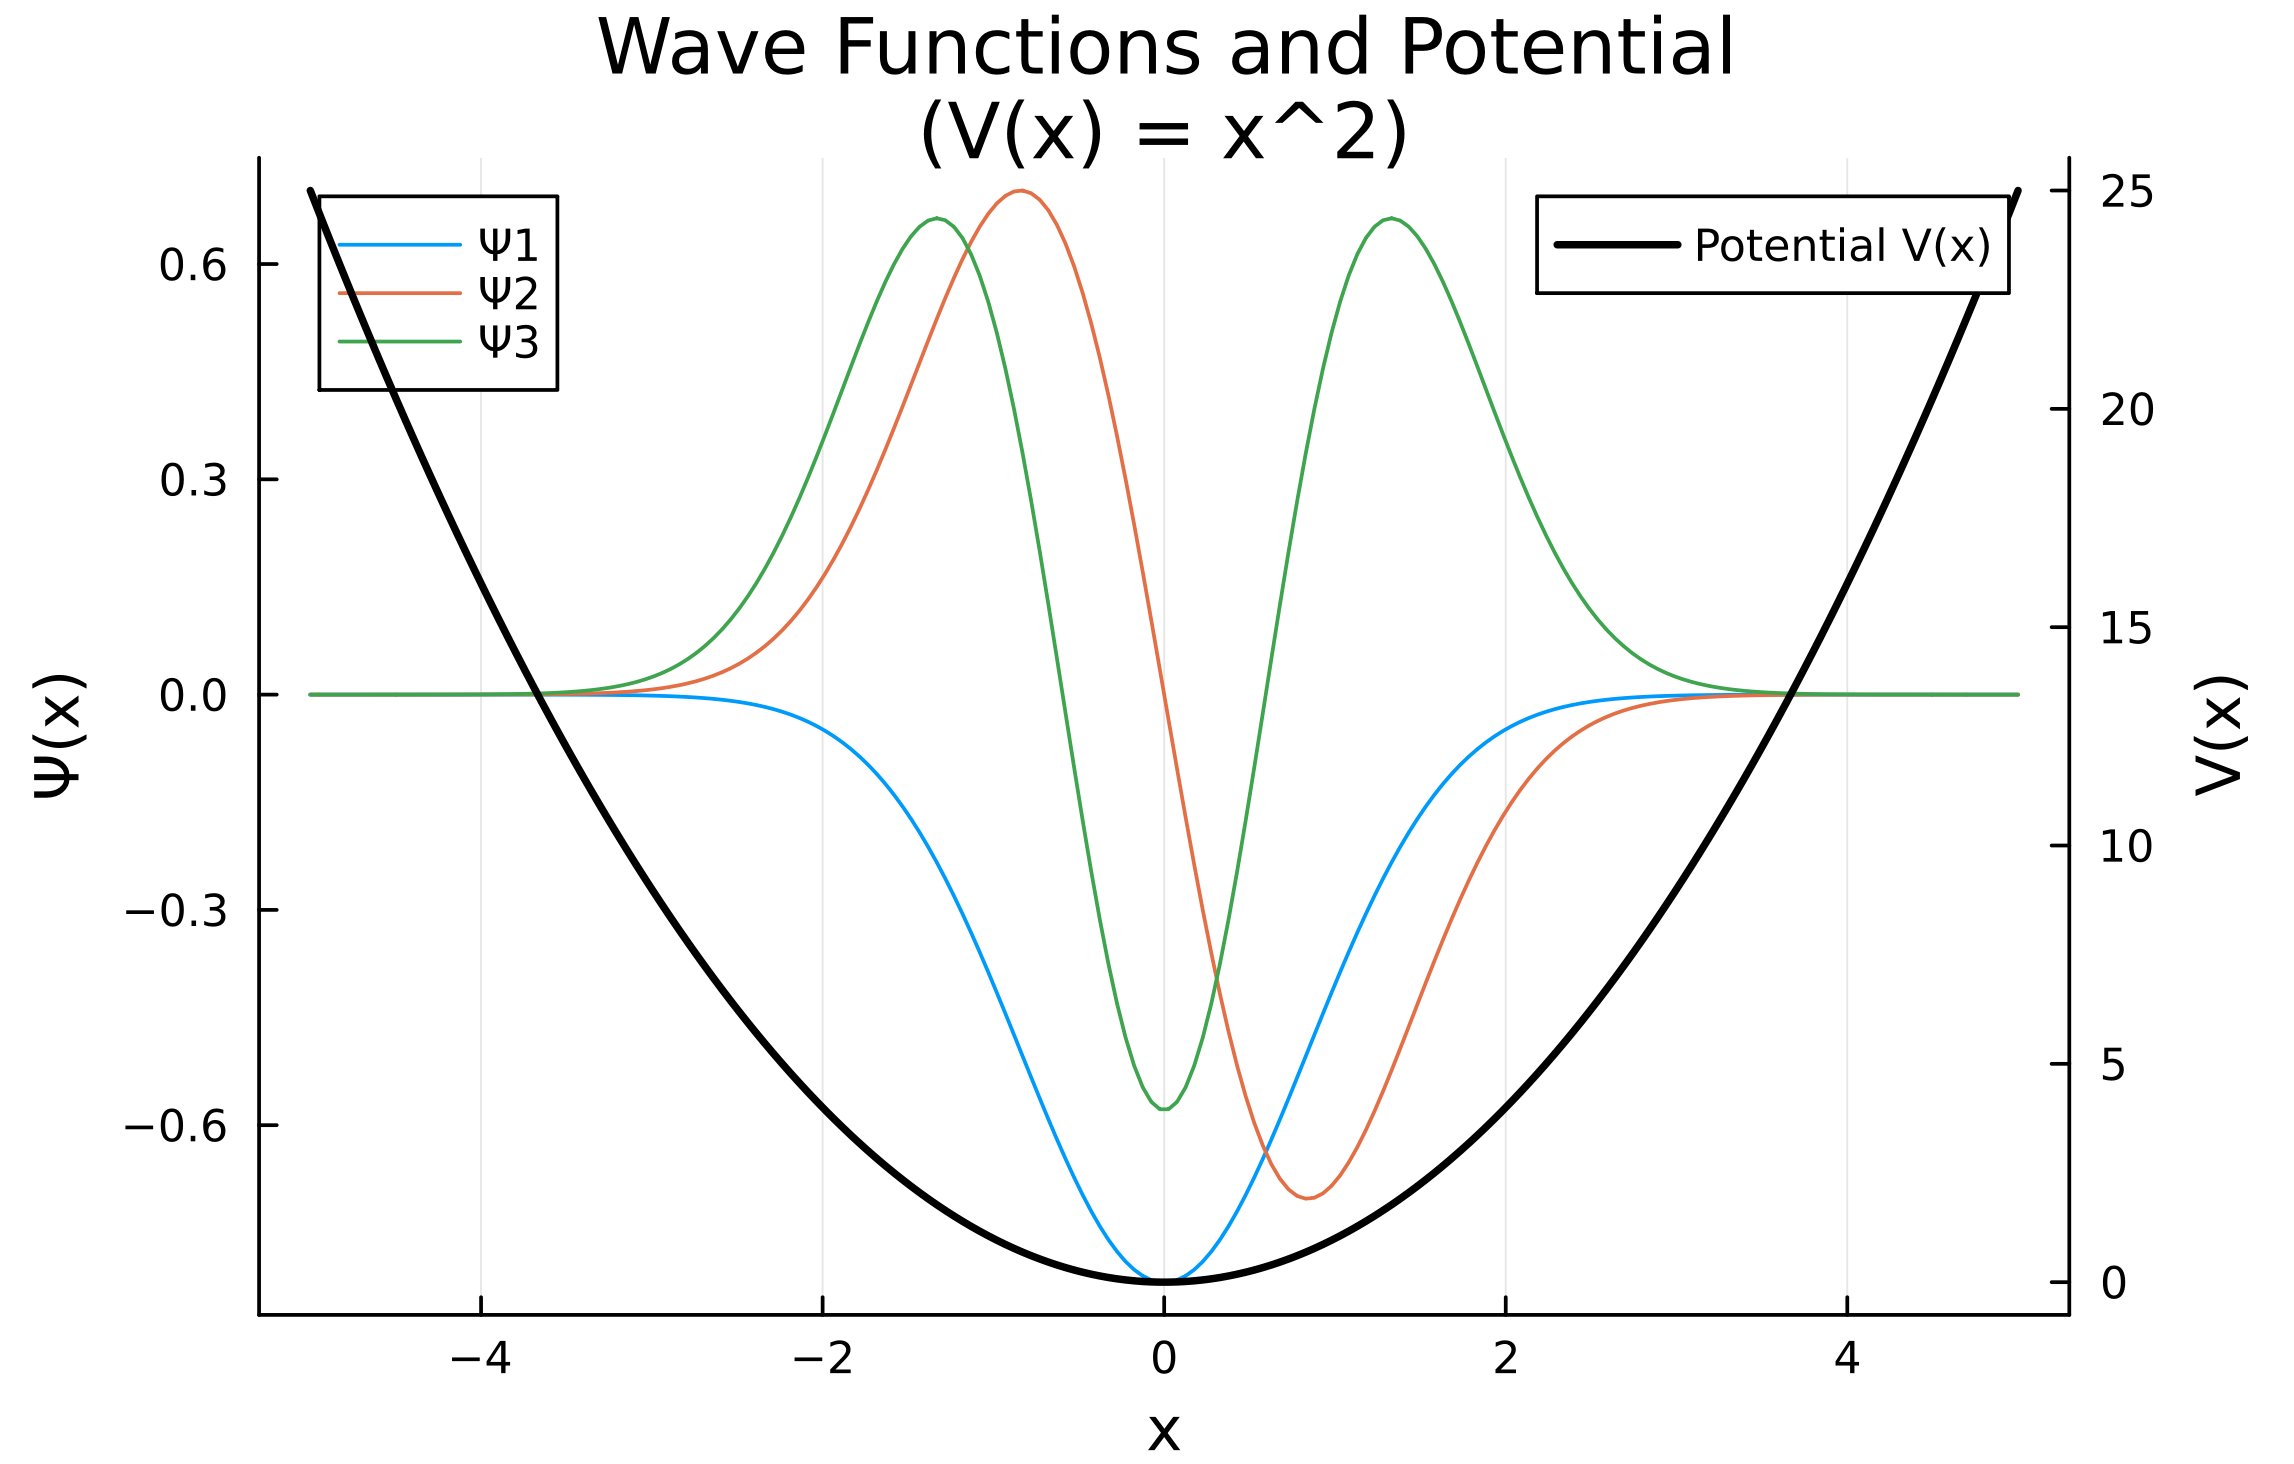
\includegraphics[width=0.5\textwidth]{Problem_3/figs/plot_1.png}
    \hspace{5pt}
    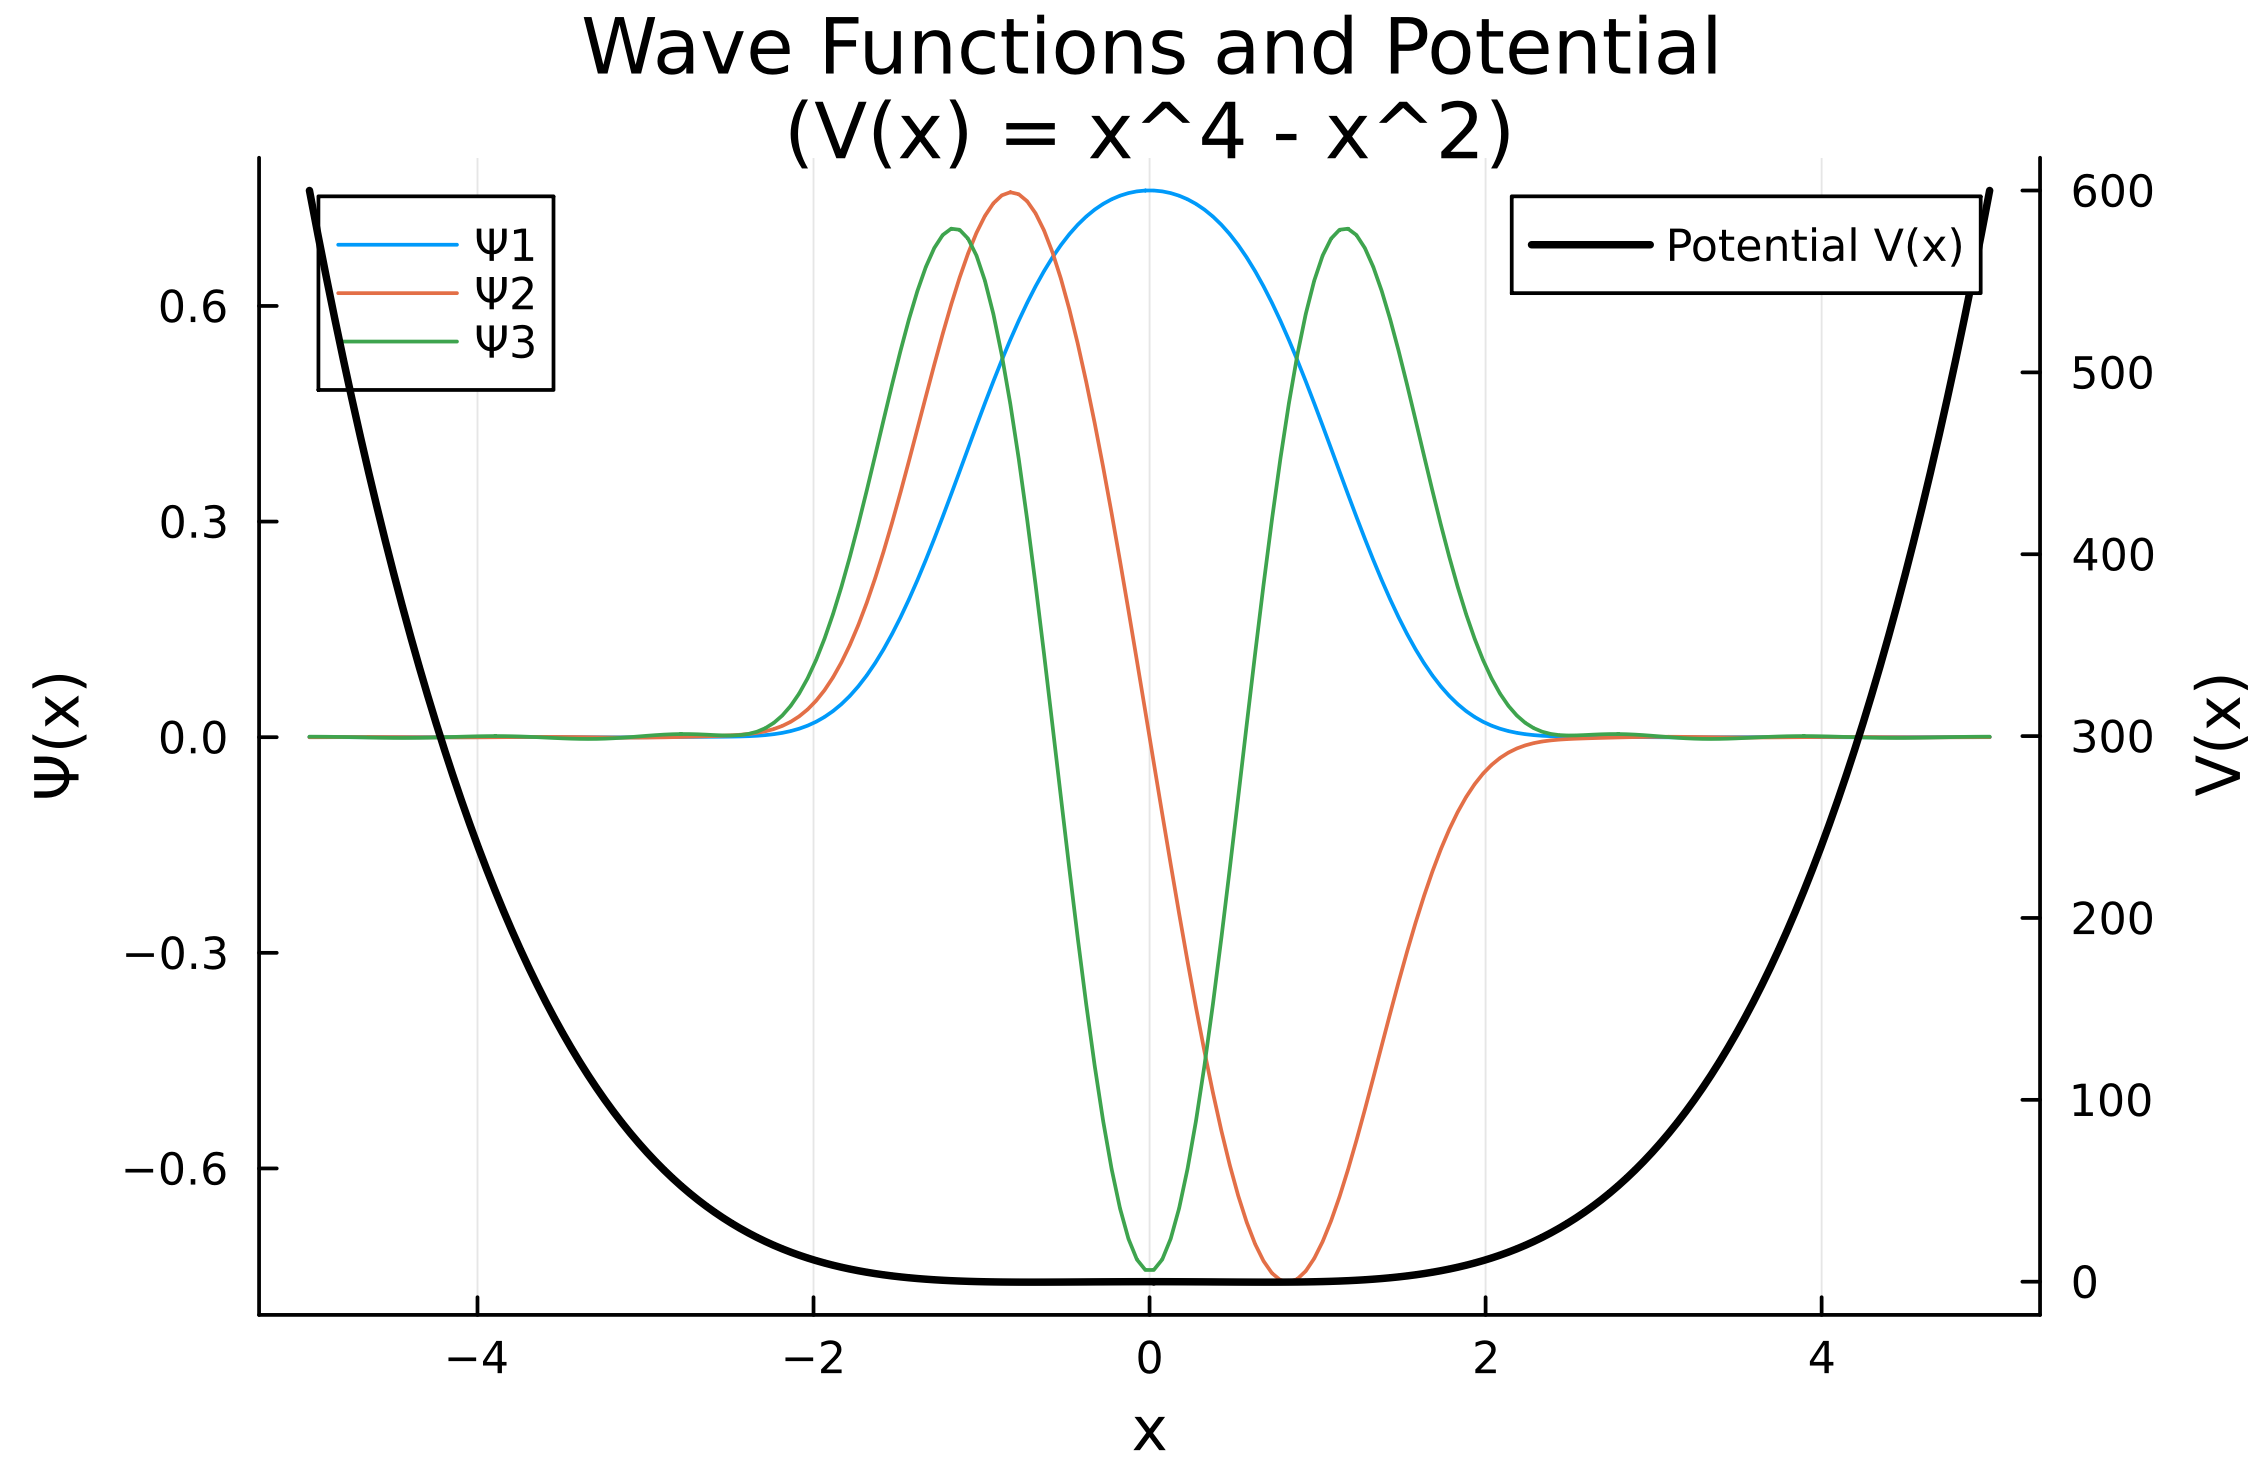
\includegraphics[width=0.5\textwidth]{Problem_3/figs/plot_2.png}
	\caption{选项3:使用默认参数求解$V=x^2$与$V=x^4-x^2$及其前$3$个能级}
\end{figure}

\begin{figure}[H]
	\centering
	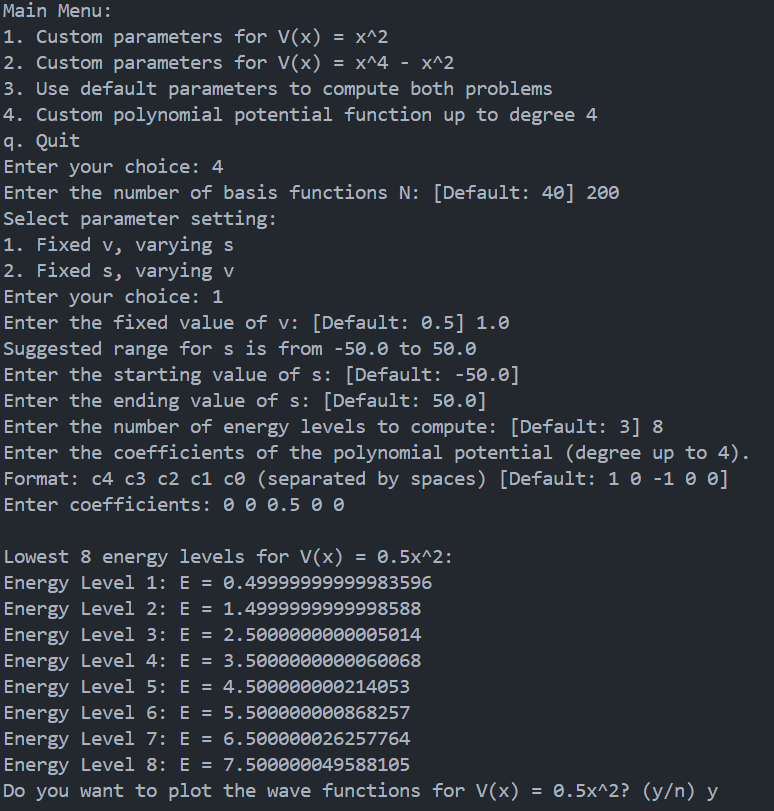
\includegraphics[width=0.75\textwidth]{Problem_3/figs/choice_4.png}
    \hspace{5pt}
    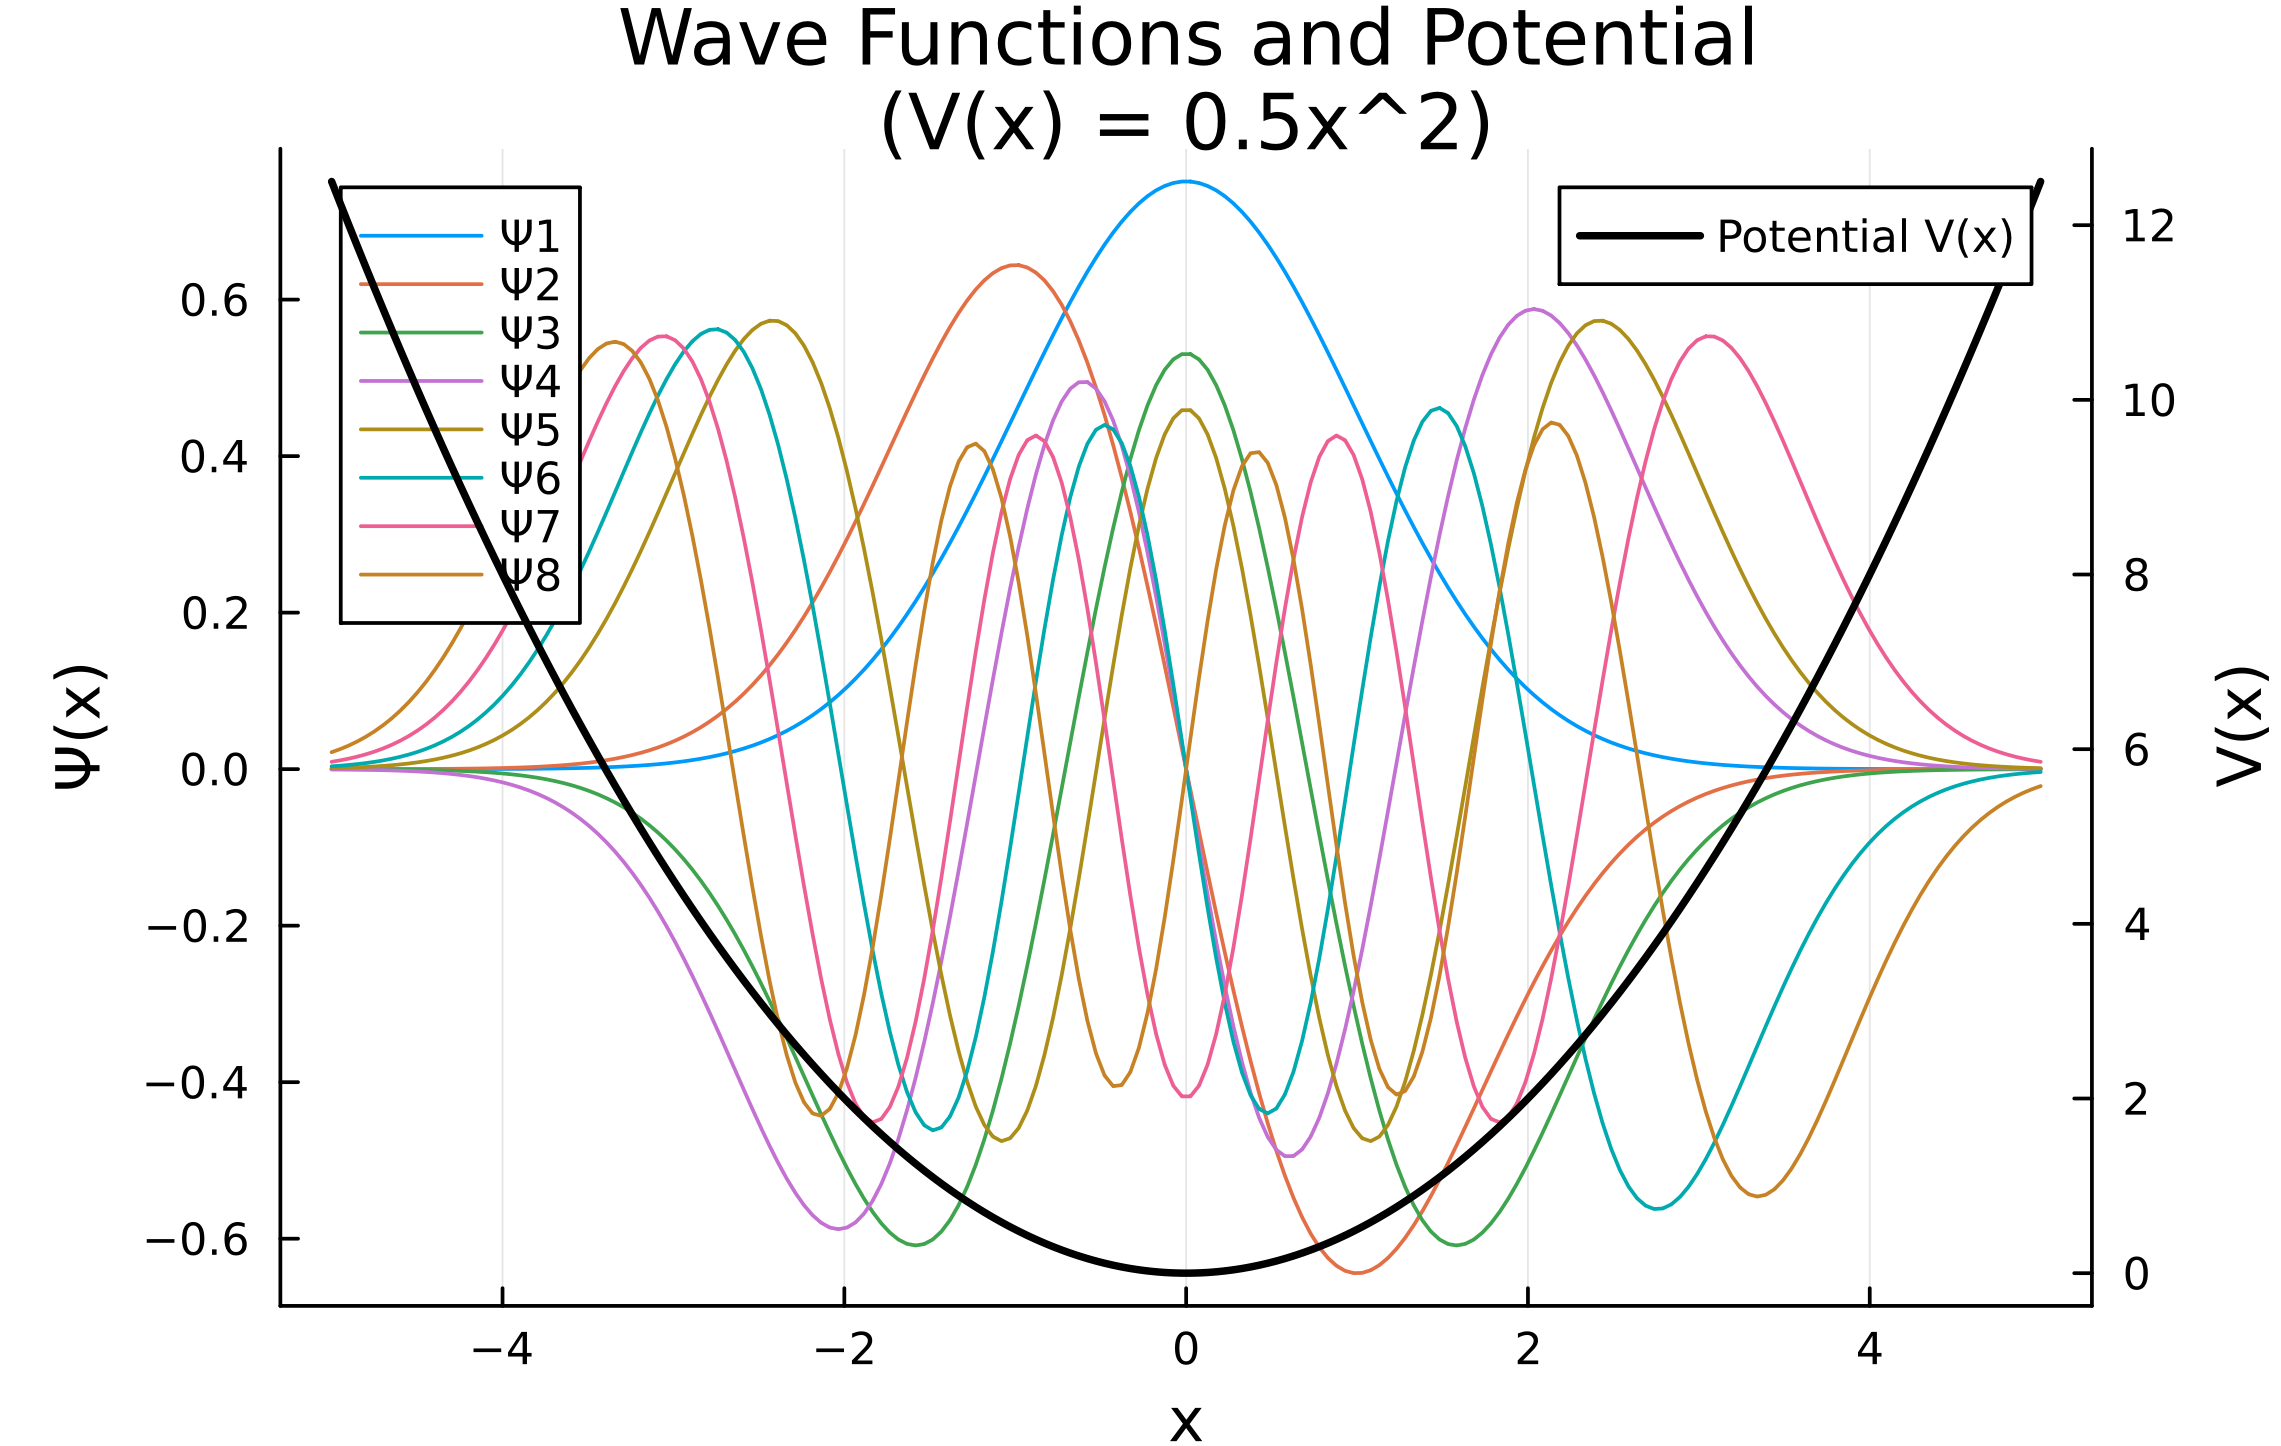
\includegraphics[width=0.75\textwidth]{Problem_3/figs/plot_3.png}
	\caption{选项4:求解自定义势阱$V=\frac{1}{2}x^2$及其前$8$个能级}
	\caption*{\footnotesize{\textbf{注:} 在自然单位制下,与解析解$E_n = (n+\frac{1}{2})\hbar \omega$数值一致}}
\end{figure}

\begin{figure}[H]
	\centering
	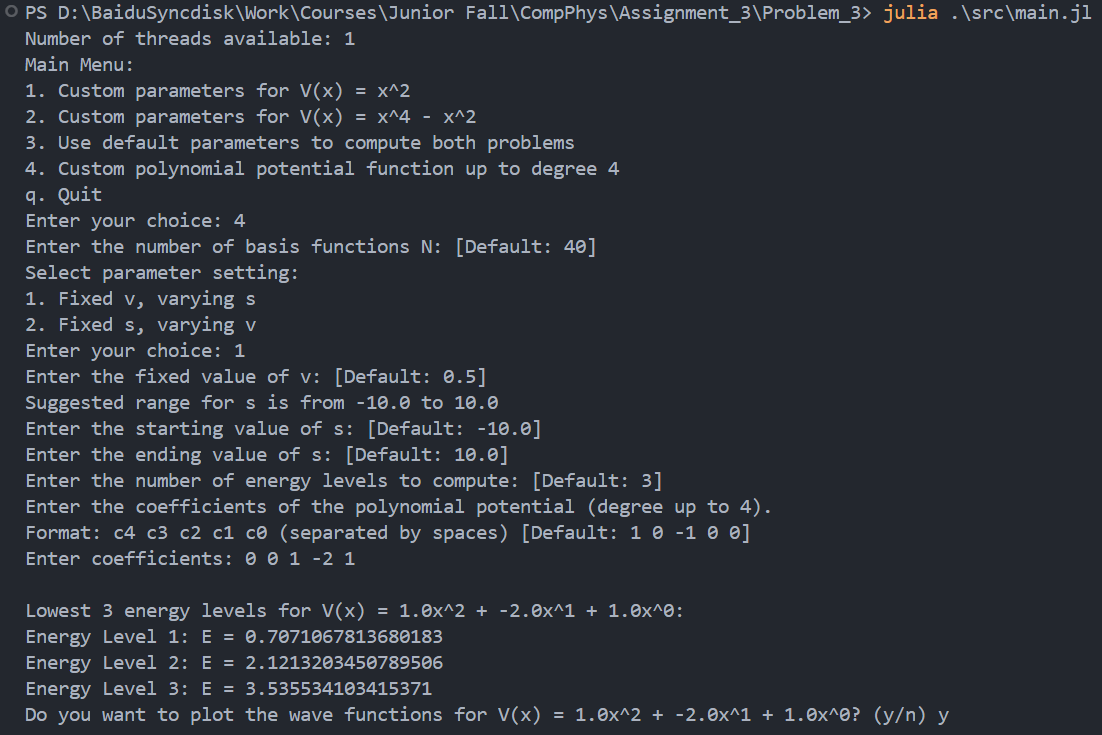
\includegraphics[width=0.8\textwidth]{Problem_3/figs/choice_4_2.png}
    \hspace{5pt}
    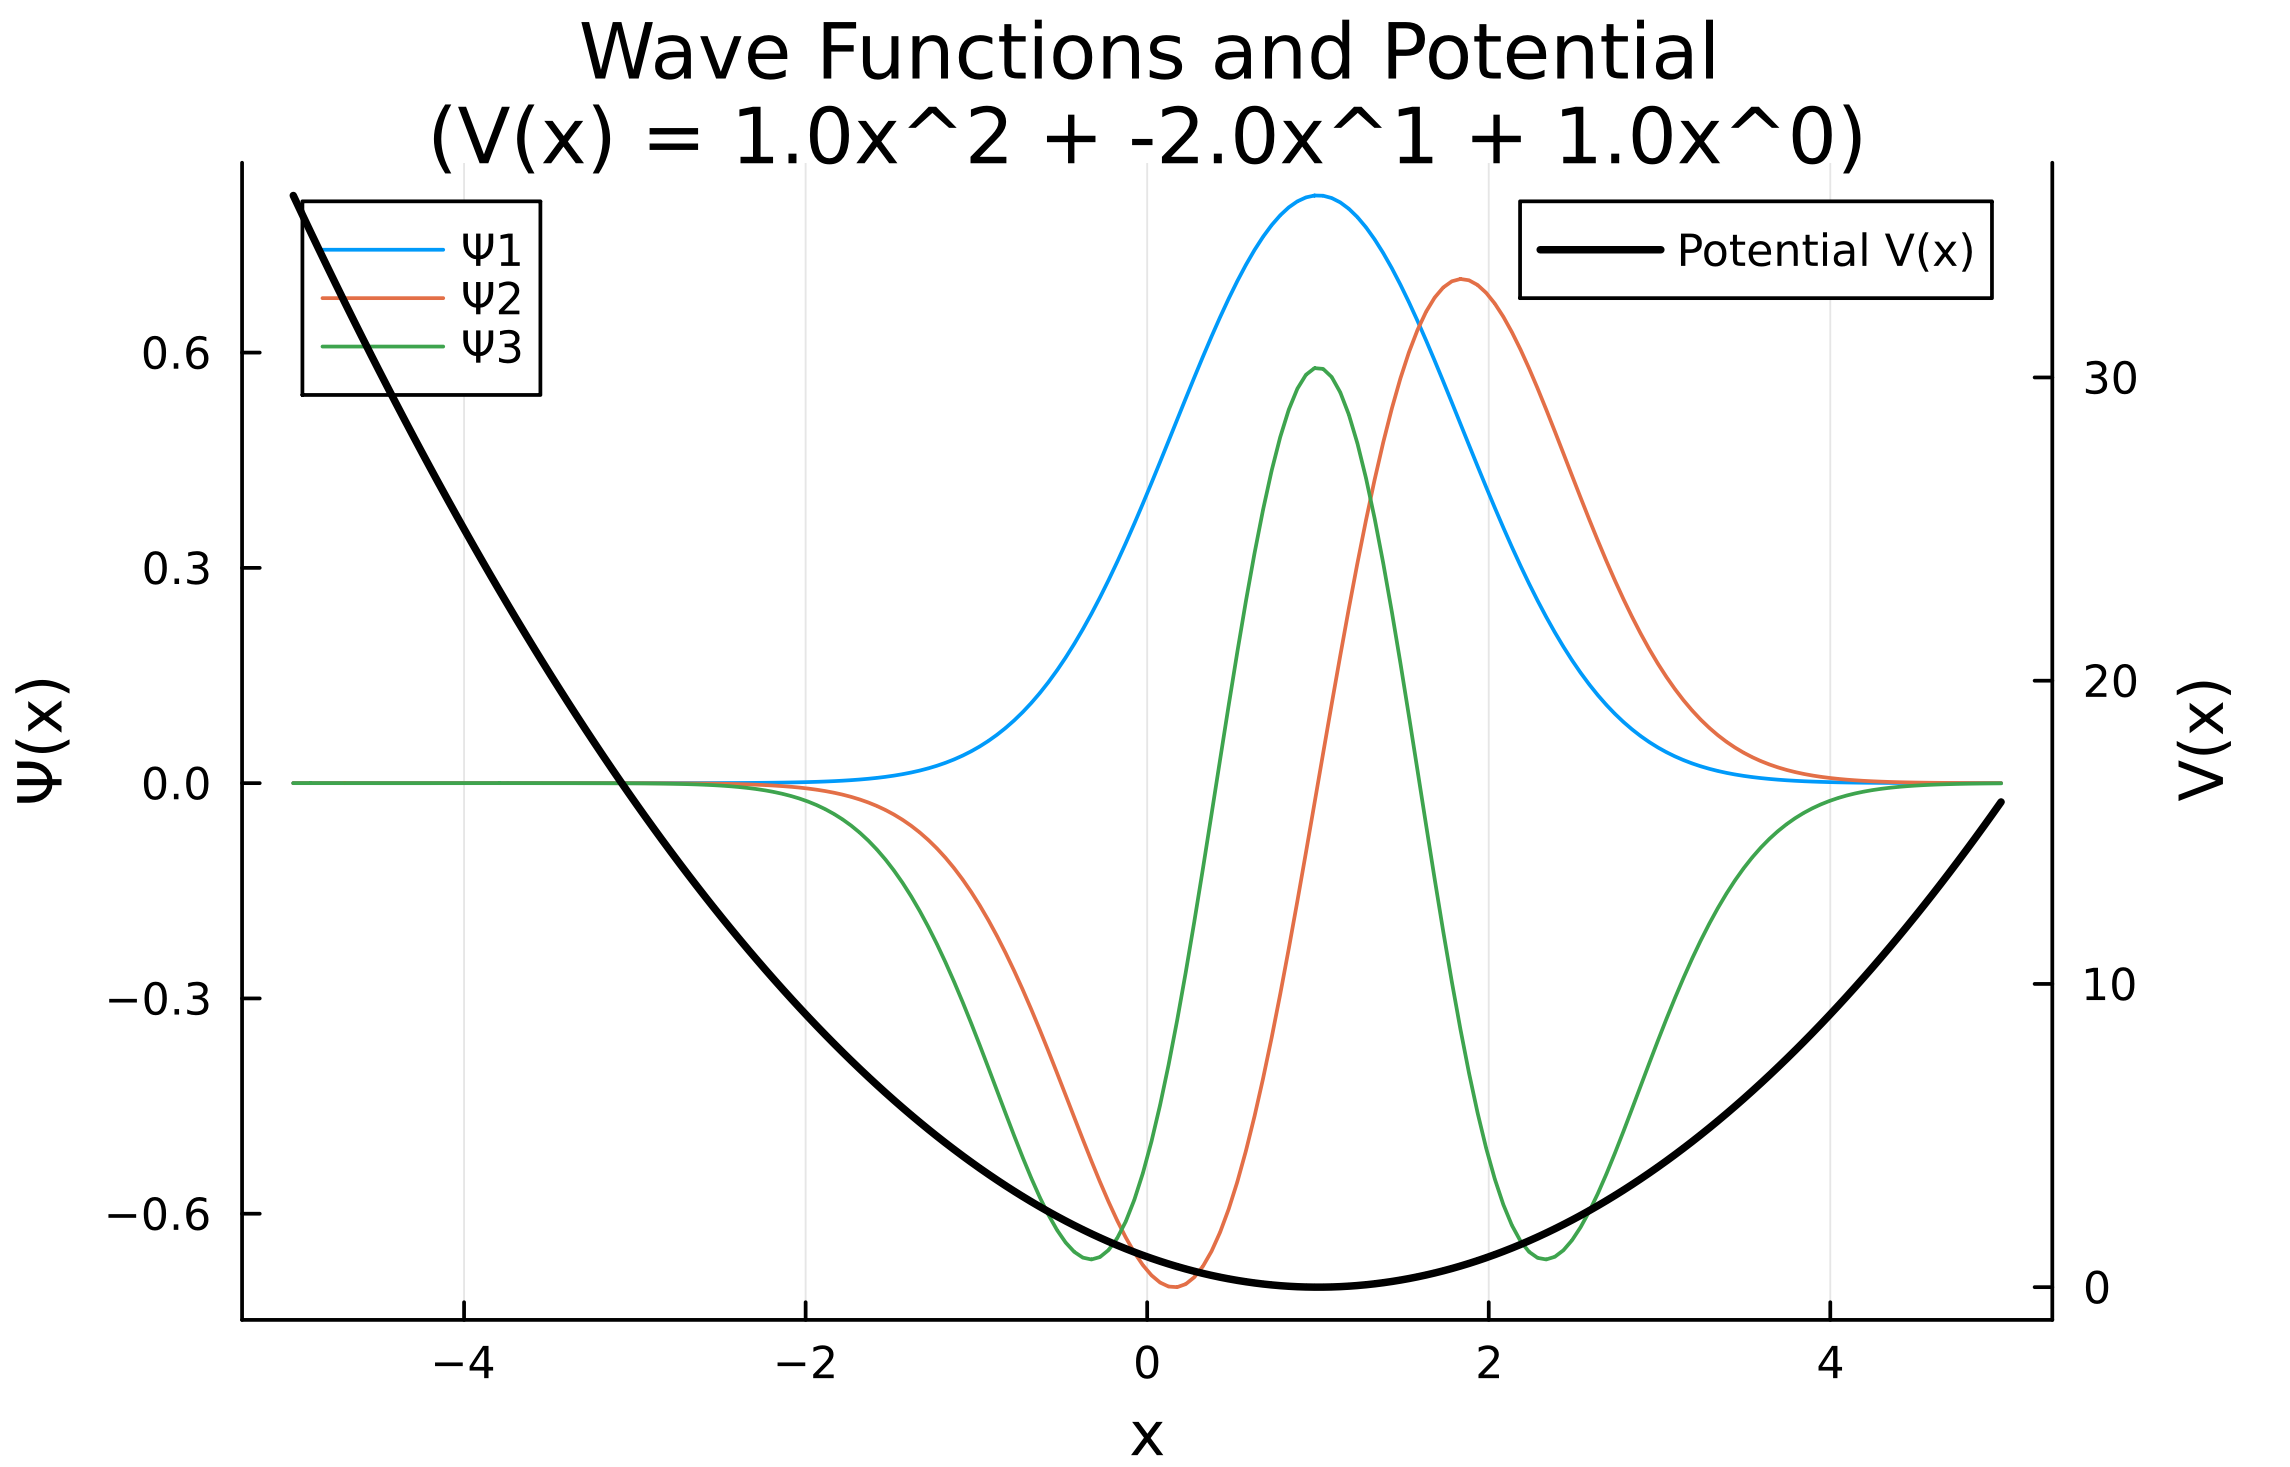
\includegraphics[width=0.8\textwidth]{Problem_3/figs/plot_4.png}
	\caption{选项4:求解自定义势阱$V=(x+1)^2$及其前$3$个能级}
	\caption*{\footnotesize{\textbf{注:} 能级与势阱$V=x^2$一致,波函数相较势阱$V=x^2$平移}}
\end{figure}

